% Dies ist Teil der Vorlesung Physik auf dem Computer, SS 2012,
% Axel Arnold, Universitaet Stuttgart.
% 
% Dieses Werk ist unter einer Creative Commons-Lizenz vom Typ
% Namensnennung-Weitergabe unter gleichen Bedingungen 3.0 Deutschland
% zugänglich. Um eine Kopie dieser Lizenz einzusehen, konsultieren Sie
% http://creativecommons.org/licenses/by-sa/3.0/de/ oder wenden Sie sich
% schriftlich an Creative Commons, 444 Castro Street, Suite 900, Mountain
% View, California, 94041, USA.

\chapter{Lineare Algebra \textrm{II}}
\index{Gleichungssysteme>lineare}
\label{chap:la}

Wie wir bereits an der Besselgleichung gesehen haben, lassen sich
gewöhnliche Differentialgleichungen in einer Dimension recht einfach
auf lineare Gleichungssysteme abbilden. Diese haben Bandstruktur und
sind effizient zu lösen.  In mehr als einer Dimension ist das
allerdings im Allgemeinen nicht mehr der Fall. Betrachten wir zum
Beispiel die Poissongleichung in zwei Dimensionen:
\begin{equation}
  \label{eq:laplace}
  \Delta \phi = \frac{\partial^2 \phi}{\partial x^2} +
  \frac{\partial^2 \phi}{\partial y^2} = \rho.
\end{equation}
Wir diskretisieren nun wie gewohnt $\phi(x,y)$ in beiden Dimensionen
zu $\phi_{k, l} = \phi(k h, l h)$, $k,l=(1)N$. Den Laplace-Operator
erhalten wir dann in erster Ordnung als
\begin{align}
  \label{eq:laplacedisc}
  \Delta \phi(k h, l h) \approx
  \frac{1}{h^2}\bigl(\phi_{k+1,l} -
  2\phi_{k,l}  + \phi_{k-1,l}\bigr) + 
  \frac{1}{h^2}\bigl(\phi_{k,l+1} -
  2\phi_{k,l}  + \phi_{k,l-1}\bigr)\nonumber\\
  = \frac{1}{h^2}\bigl(
  \phi_{k,l+1} + \phi_{k+1,l} - 4\phi_{k,l} +
  \phi_{k-1,l} + \phi_{k,l-1}\bigr).
\end{align}
Der Einfachheit halber nehmen wir periodische Randbedingungen an, so
dass wir diese Gleichung für jeden Gitterpunkt aufstellen
können. Allerdings wäre die resultierende Matrix singulär; um die
Differenzialgleichung mit periodischen Randbedingungen eindeutig lösen
zu können, müssen wir einen Funktionswert vorgeben.

Diese Gleichungen sind im Moment noch auf der Matrix $\phi_{k,l}$
definiert, die wir nun \emph{linearisieren} müssen, um die Gleichung
in der gewohnten Matrixform etwa an Python zu übergeben. Hierzu
speichern wir die Elemente von $\phi_{k,l}$ wie folgt:
\begin{equation}
  \Phi_{k + N l} = \phi_{k,l} \quad\text{für}\; k,l=1(1)N.
\end{equation}
Wie man sich leicht überlegt, ist diese Zuordnung eindeutig, wir
können also beliebig zwischen $\Phi_n$ und $\phi_{k,l}$ wechseln und
so etwa \eqref{eq:laplacedisc} auf den Vektor $\Phi_n$
übertragen. Dies ergibt dann $N^2$ Gleichungen für alle Datenpunkte,
die in Matrixform für $N=5$ zum Beispiel wie folgt aussehen:
\begin{equation}
  \label{eq:2d-laplace}
  \left( \text{\raisebox{-4\baselineskip}{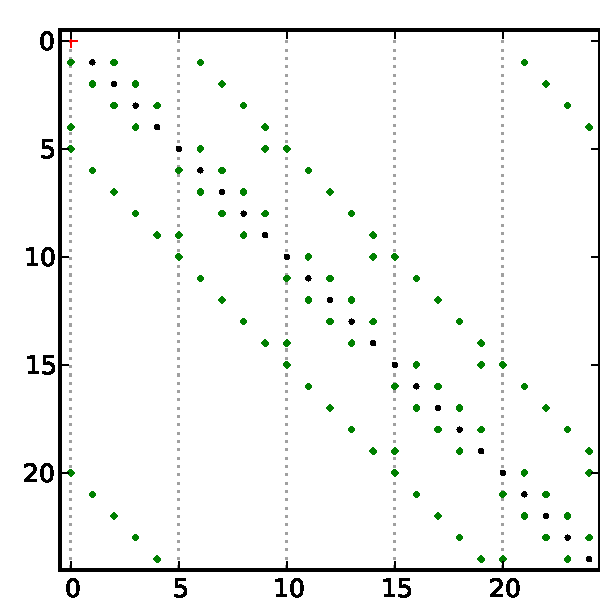
\includegraphics[height=8.5\baselineskip]{plots/2d-laplace}}} \;\right)
  \;\cdot\begin{pmatrix}
    \Phi_0 = \phi(0,0)\\
    \Phi_1 = \phi(h,0)\\
    \vdots\\
    \Phi_{4} = \phi(h,0)\\
    \Phi_{5} = \phi(0,h)\\
    \vdots\\
    \Phi_{24} = \phi(4h,4h)
  \end{pmatrix}
  =
  \begin{pmatrix}
    \Phi_0\\
    \rho(h,0)\\
    \vdots\\
    \rho(h,0)\\
    \rho(0,h)\\
    \vdots\\
    \rho(4h,4h)
  \end{pmatrix}
  .
\end{equation}
In der Matrix markieren grüne Punkte Einträge mit Wert $1/h^2$,
schwarze Punkte Einträge mit Wert $-4/h^2$ und das rote Kreuz den
Normierungseintrag mit Wert 1. Alle anderen Einträge sind Null.

Durch die periodischen Randbedingungen in $x$ und $y$ sind zwei
Nebendiagonalen weiter außen teilweise besetzt. Damit hat die
entstehende Matrix zwar immer noch Bandstruktur hat und ist dünn
besetzt, \dh fast alle Einträge Null, allerdings ist sie nicht mehr
tridiagonal. Auch durch Umsortieren lässt sich dies nicht wesentlich
ändern, daher muss die volle Gaußelimination durchgeführt werden. Für
Gitter von $5\times 5$ Punkten ist das zwar noch unproblematisch, bei
einem Gitter von $100\times 100$ Punkten hat die volle Matrix
allerdings bereits $100,000,000$ Einträge, und die Gaußelimination
wird zu langsam. Noch schwieriger wird es in den meist benutzten
drei Dimensionen, da die volle Matrix schnell mehrere Milliarden
Einträge hat.

Neben der Ineffizienz des Gaußverfahrens bringt das Arbeiten mit der
vollen Matrix allerdings auch Speicherprobleme mit sich, denn eine
volle Matrix aus dem $\RR^{100,000\times 100,000}$ benötigt bei
einfacher Genauigkeit über 37GB Speicher. Dünn besetzte Matrizen
dieser Größe sind allerdings durchaus handhabbar, denn nur wenige
Matrixelemente sind überhaupt ungleich Null. Indem man nur diese
Elemente geschickt speichert, lassen sich sogar noch weitaus größere
Matrizen bewältigen. Auf derartigen Datenstrukturen kann die
Gaußelimination allerdings nicht effizient eingesetzt werden, da diese
die Matrixstruktur durch die Zeilenadditionen rasch zerstört.

Im Folgenden lernen wir nun schnellere, iterative Gleichungslöser
kennen, mit denen auch solche und größere Gleichungssysteme handhabbar
werden. Außerdem können diese Verfahren auch auf große, dünn besetzte
Matrizen angewandt werden. Weiter lernen wir die QR-Zerlegung als
weitere Matrixzerlegung kennen, die eine wichtige Rolle bei der
Bestimmung von orthogonalen Basen und der 
Optimierung spielt. Sie kann auch zur Berechnung von Eigenwerten und
-vektoren benutzt werden, was dieses Kapitel abschließt.

\section{Iterative Gleichungslöser}

Wir betrachten eine reguläre Matrix $A\in\RR^{n,n}$ und einen Vektor
$b\in\RR^n$. Gesucht ist dann die Lösung $\overline{x}\in\RR^n$ mit
\begin{equation}
  \label{eq:axb}
  A\overline{x} = b.
\end{equation}

Die Gaußelimination liefert diese bei unendlicher Genauigkeit exakt,
allerdings mit dem hohen Aufwand $\O(n^3)$. Wir haben allerdings
bereits gesehen, dass iterative Verfahren wie etwa das Newtonverfahren
zur Lösung nichtlinearer Gleichungssysteme quadratisch
konvergieren. Hierzu gibt es mehrere mögliche Ansätze, etwa das
CG-Verfahren, das auf einem Optimierungsproblem beruht und das wir
später kennenlernen werden. Zunächst suchen wir aber iterative
Verfahren der Form
\begin{equation}
  \label{eq:itgl}
  x^{(i+1)} = G(x^{(i)}) = T x_i + r
\end{equation}
mit $r\in\RR^n$ und $T\in\RR^{n,n}$, $\norm{T}<1$. Der Banachsche
Fixpunktsatz gewährleistet, dass diese sukzessive Substitution für
jeden Startwert konvergiert, wobei die Norm $\norm{\cdot}$ wiederum
geeignet gewählt werden kann.

Wie müssen wir nun $T$ wählen, damit einerseits $x^{(i)}\to \overline{x}$
für $i\to\infty$, andererseits aber $T$ und $r$ einfach zu berechnen
sind? Da $\norm{T} < 1$ sein soll, muss $r$ bereits eine
Näherungslösung sein. Es sollte also $r = B^{-1}b$ sein, wobei $B$
eine geeignete, einfach zu invertierende Näherung von $A$ ist. Dann
gilt
\begin{equation}
  \overline{x} = T\,\overline{x} +
  B^{-1}b
  \stackrel{!}{=} T\,\overline{x} +
  B^{-1}A\,\overline{x}
  = \left(T + B^{-1}A\right)\overline{x},
\end{equation}
was sich offenbar durch Wahl von $T = I - B^{-1}A$ erfüllen
lässt. Solange also $B^{-1}$ einfach zu bestimmen ist, lassen sich
sowohl $T$ als auch $r$ einfach berechnen.

\subsection{\keyword{Jacobiverfahren}}

Das erste Verfahren nach diesem Schema, dass wir kennenlernen, ist
das Jacobiverfahren. Die Matrix $A$ wird dazu als Summe einer
Diagonalmatrix sowie einer linken, unteren und einer rechten oberen
Dreiecksmatrix mit verschwindender Diagonale zerlegt, also $A = L + D
+ U$ mit
\begin{equation}
  l_{ik}=
  \begin{cases}
    a_{ik} & \text{für}\; i<k\\
    0 & \text{sonst}
  \end{cases},\quad
  d_{ik} =
  \begin{cases}
    a_{ik} & \text{für}\; i=k\\
    0 & \text{sonst}
  \end{cases}\quad\text{und}\;
  u_{ik} =
  \begin{cases}
    a_{ik} & \text{für}\; i>k\\
    0 & \text{sonst}
  \end{cases}.
\end{equation}
Die Diagonalmatrix $D$ soll dabei die Rolle der leicht zu
invertierenden Matrix übernehmen. Dazu müssen die Diagonalelemente
alle von Null verschieden sein, was sich bei einer regulären Matrix
$A$ durch Vertauschen von Zeilen und/oder Spalten immer erreichen
lässt.

Setzen wir also $T=I-D^{-1}A$ und $r=D^{-1}b$ in \eqref{eq:itgl} ein,
so erhalten wir das \emph{Jacobiverfahren}
\begin{align}
  x^{(i+1)} = \left(I - D^{-1}A\right)x^{(i)} + D^{-1}b\nonumber\\
  = -D^{-1}\left(L + U\right)x^{(i)} + D^{-1}b
\end{align}
mit der Diagonalmatrix $D$, so dass $d^{-1}_{jj} =
\frac{1}{a_{jj}}$. Komponentenweise bedeutet dies, dass
\begin{equation}
  \label{eq:jacobicomp}
  x_j^{(i+1)} = \frac{1}{a_{jj}}\left(b_j - \sum_{k\neq j} a_{jk}x_k^{(i)}\right).
\end{equation}
Mit anderen Worten, dass Jacobiverfahren löst jede Zeile nach der
Variablen auf der Diagonale auf.

\index{strikt diagonaldominant}
Wann konvergiert dieses Verfahren? Eine gängige Voraussetzung ist,
dass die Matrix $A$ strikt diagonaldominant ist, also
\begin{equation}
  \sum_{k\neq i} \abs{a_{ik}} < \abs{a_{ii}}\quad\text{für}\; i=1(1)n.
\end{equation}
Diese Bedingung ist sehr stark, zum Beispiel erfüllen weder die Matrix
aus dem Eingangsbeispiel noch etwa die für die Spline-Interpolation
benötigten Matrizen diese Bedingung, da in beiden Fällen das
Diagonalelement betragsmäßig die Summe der Nebenelemente
ist. Allerdings sind die bei der sogenannten Finite-Elemente
Modellierung zur Diskretisierung von Differentialgleichungen
entstehenden Matrizen meist strikt diagonaldominant. Daher spielen
Löser für diese Art von Matrizen auch kommerziell eine wichtige Rolle.

Ist $A$ strikt diagonaldominant, so nutzen wir die Maximumsnorm
\begin{equation}
  \norm{A}_\infty := \max_{i=1}^n \sum_{k=1}^n \abs{a_{ik}},
\end{equation}
die eine Matrixnorm definiert. Dann gilt
\begin{equation}
  \norm{T}_{\infty} = \norm{I-D^{-1}A}_{\infty} =
  \max_{i=1}^n \sum_{k\neq i} \frac{\abs{a_{ik}}}{\abs{a_{ii}}} < 1,
\end{equation}
die sukzessive Substitution und damit das Jacobiverfahren konvergieren
also. Außerdem ist die Konvergenz linear, genauer gilt
\begin{equation}
  \frac{\norm{x_{n+1} - \overline{x}}_\infty}{\norm{x_{n} - \overline{x}}_\infty}
  \le \sum_{k\neq i} \frac{\abs{a_{ik}}}{\abs{a_{ii}}},
\end{equation}
wobei $\norm{x}_\infty := \max_{i=1}^n \abs{x_i}$ die
Vektormaximumsnorm bezeichnet. Je größer also die Diagonaleinträge
gegenüber den Nebeneinträgen sind, desto schneller konvergiert das
Verfahren, zum Beispiel wenn die Matrix eine kleine Störung der
Einheitsmatrix ist.

\subsubsection{Indizierte Matrixspeicherung}
\index{indizierte Matrixspeicherung}
\index{Indexformat}

Wie man an der komponentenweisen Darstellung \eqref{eq:jacobicomp} gut
sieht, kann das Jacobiverfahren auch auf dünnbesetzten Matrizen
implementiert werden. Zum einen wird die Matrix $A$ beim Verfahren
nicht verändert, sondern nur der erheblich kleinere Lösungsvektor, zum
anderen wird nur zeilenweise summiert, was eine indizierte Speicherung
ermöglicht.  Dazu wird für jede Zeile $j$ lediglich der
Diagonaleintrag $a_{jj}$ explizit gespeichert, sowie eine Liste mit
Einträgen $(k, a_{jk})$, die die restlichen Elemente $\neq 0$
enthält. Eine Implementation des Jacobiverfahrens muss dann lediglich
für jede Zeile die Summe $\sum_{k\neq j} a_{jk}x_k^{(i)}$ mit
Hilfe der zur Zeile gehörigen Liste bilden, von $b_j$ abziehen und
durch $a_{jj}$ teilen.

In unserem einführenden Beispiel wären pro Zeile neben der Diagonalen
maximal vier weitere Einträge nötig, unabhängig davon, wie fein die
Schrittweite gewählt wird. Die Matrix \eqref{eq:2d-laplace} würde
damit so dargestellt:
{\small
  \begin{align}
    1, \{\} \;&\mathop{\widehat{=}}\; \left(1, 0, \ldots, 0\right)
    \nonumber\\
    -\frac{4}{h^2}, \left\{
      \left(3, \frac{1}{h^2}\right), \left(1, \frac{1}{h^2}\right),
      \left(7, \frac{1}{h^2}\right), \left(22, \frac{1}{h^2}\right)
    \right\}
    \;&\mathop{\widehat{=}}\;
    \left(\frac{1}{h^2}, -\frac{4}{h^2}, \frac{1}{h^2}, 0, 0, 0, 1, 0,
      \ldots, 0, 1, 0, 0, 0\right)\nonumber\\
    -\frac{4}{h^2}, \left\{
      \left(4, \frac{1}{h^2}\right), \left(2, \frac{1}{h^2}\right),
      \left(8, \frac{1}{h^2}\right), \left(23, \frac{1}{h^2}\right)
    \right\}
    \;&\mathop{\widehat{=}}\;
    \left(0, \frac{1}{h^2}, -\frac{4}{h^2}, \frac{1}{h^2}, 0, 0, 0, 1, 0,
      \ldots, 0, 1, 0, 0\right)\nonumber\\
    &\vdots\\
    a_{jj}, \left\{(k_1, a_{jk_1}),(k_2, a_{jk_2}), \ldots\right\}
    \;&
  \end{align}}

\subsection{\keyword{Gauß-Seidel-Verfahren}}

Wird \eqref{eq:jacobicomp} zeilenweise abgearbeitet, so müssen die
bereits berechneten Werte $x_j^{(i+1)}$ zwischengespeichert werden,
da für die restlichen Zeilen ja noch die alten Werte $x_k^{(i)}$
benötigt werden. Beim Gauß-Seidel-Verfahren werden stattdessen die
bereits berechneten, neueren Werte benutzt:
\begin{equation}
  \label{eq:gscomp}
  x_j^{(i+1)} = \frac{1}{a_{jj}}\left(b_j -
    \sum_{k=1}^{j-1} a_{jk}x_k^{(i+1)} - \sum_{k=j+1}^n a_{jk}x_k^{(i)}\right).
\end{equation}
Dies erspart einerseits die getrennte Speicherung der neuen
Näherungslösung $x_k$, andererseits ist die neue Näherungslösung näher
an der Lösung, so dass es durchaus sinnvoll erscheint, diese neuen, besseren
Werte für die verbleibenden Zeilen zu nutzen.

Mit der Zerlegung $A=L + D + U$ wie beim Jacobiverfahren ergibt sich
in Matrixschreibweise
\begin{equation}
  x^{(i+1)} = -D^{-1}L x^{(i+1)} - D^{-1} U x^{(i)} + D^{-1}b
  \;\implies\;
  (D + L)x^{(i+1)} = - U x^{(i)} + b
\end{equation}
und damit
\begin{equation}
  x^{(i+1)} = -(D+L)^{-1} U x^{(i)} - (D+L)^{-1}b.
\end{equation}
Das Gauß-Seidel-Verfahren ist also auch vom Typ \eqref{eq:itgl}, mit
der etwas komplexeren Matrix $B= D + L$. Tatsächlich ist auch
\begin{equation}
  \label{eq:gst}
  T = I - (D + L)^{-1} A = (D + L)^{-1}(D + L - A) = -(D+L)^{-1} U.
\end{equation}
Man kann zeigen, dass $\norm{T}_\infty$ beim Gauß-Seidel-Verfahren
kleiner ist als beim Jacobi-Verfahren. Das bedeutet allerdings im
allgemeinen nicht, dass das Gauß-Seidel-Verfahren schneller ist, trotz
dessen, dass teilweise mit prinzipiell besseren Näherungen gerechnet
wird. Man spart allerdings den Speicherplatz, um $x^{(i+1)}$
zwischenzuspeichern.

Genauso wie das Jacobiverfahren kann auch das Gauß-Seidel-Verfahren
auf indizierten Matrixformaten benutzt werden, wobei die beiden Summen
in \eqref{eq:gscomp} entweder gleichzeitig aufaddiert werden, oder die
Listen der Nichtdiagonalelemente in Elemente links und rechts der
Diagonalen aufgeteilt.

Insbesondere für die parallele Verarbeitung, die mit der heutigen
weiten Verbreitung von Mehrkern-Prozessoren ein wichtiger Faktor ist,
ist das Gauß-Seidel-Verfahren allerdings ungeeignet, da die Berechnung
jeder Zeile die Ergebnisse der vorherigen erfordert. Das
Jacobi-Verfahren kann hingegen auf so viele Prozessoren verteilt
werden, wie die Matrix Zeilen hat, was eine effiziente Verarbeitung
selbst auf modernen Grafikkarten ermöglicht.

\subsection{\keyword{Relaxationsverfahren}}
\index{Successive over-relaxation}
\index{SOR}

Beim Relaxationsverfahren (Successive over-relaxation, SOR) wird statt
$B = D + L$ die Matrix $B = D/\omega + L$ mit einem Relaxationsfaktor
$\omega$ betrachtet. Durch geeignete Wahl von $\omega$ können dann
auch nicht strikt diagonaldominante Matrizen behandelt
werden. Allerdings kann man nur zeigen, dass $0<\omega< 2$ gelten
muss, aber ein Wert $\omega$, der zu schneller Konvergenz führt, muss
durch Ausprobieren gefunden werden.

\begin{figure}
  \centering
  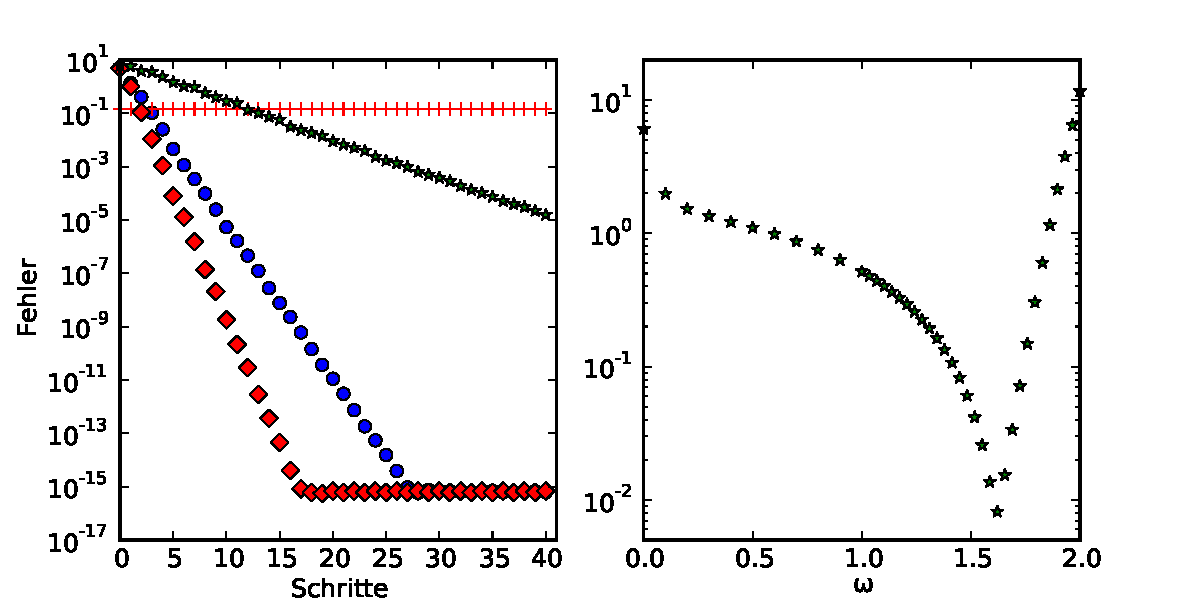
\includegraphics[width=\textwidth]{plots/iterative}
  \caption{Konvergenz von Jacobi-, Gauß-Seidel- und
    Relaxationsverfahren. Zum einen wird die Matrix $A$ aus
    \eqref{eq:2d-laplace} betrachtet, die wie gesagt nicht strikt
    diagonaldominant ist. Zum anderen wird eine Matrix $B$ mit
    genausovielen, normalverteilten Einträgen, betrachtet, die strikt
    diagonaldominant gemacht wurde, indem $b_{i,i} = 1+ \sum_{k\neq
      i}\abs{b_{ik}}$ gesetzt wurde. Links sind die Fehler
    $\norm{Bx-b}_2$ von Jacobi- und Gauß-Seidel-Verfahren für die
    Matrix $B$ mit blauen Punkten bzw.\ roten Rauten eingezeichnet. Die
    roten Kreuze zeigen hingegen den Fehler des Gauß-Seidel-Verfahrens
    für die Matrix $A$, das nicht konvergiert. Grüne Sterne
    schließlich zeigen den Fehler des SOR-Verfahrens, das mit
    $\omega=1,63$ auch bei Matrix $A$ konvergiert. Der rechte Graph
    zeigt den Fehler des SOR-Verfahrens in Abhängigkeit von $\omega$
    nach 20 Schritten.}
  \label{fig:sor}
\end{figure}

In Matrixschreibweise gilt analog zu \eqref{eq:gst}
\begin{multline}
  T = I - \omega(D + \omega L)^{-1} A =\\
  (D + \omega L)^{-1}(D + \omega L - \omega A) = -(D+\omega L)^{-1}
  \left[\omega U + (\omega-1) D\right]
\end{multline}
und damit
\begin{equation}
  x^{(i+1)} = -(D+\omega L)^{-1}
  \left[\omega U + (\omega-1) D\right]x^{(i)} +
  \omega(D + \omega L)^{-1} b
\end{equation}
beziehungsweise, analog zum Gauß-Seidel-Verfahren,
\begin{equation}
  x^{(i+1)} = -\omega D^{-1}L x^{(i+1)}
  -\left[\omega D^{-1}U + (\omega-1)I\right]x^{(i)} +
  \omega D^{-1}b.
\end{equation}
In Komponentenschreibweise schließlich ergibt sich
\begin{equation}
  x_j^{(i+1)} = \frac{\omega}{a_{jj}}\left(
    b_j
    - \sum_{k=1}^{j-1} a_{jk} x_k^{(i+1)}
    - \sum_{k=j+1}^{n} a_{jk} x_k^{(i)}\right)
  + (1-\omega) x_j^{(i)}.
\end{equation}
Das SOR-Verfahren mit $\omega=1$ entspricht also genau dem
Gauß-Seidel-Verfahren. Andere Werte von $\omega$ gewichten zwischen
der vorherigen Näherung und der nächsten
Gauß-Seidel-Iterierten. Insofern ist es erstaunlich, dass auch Werte
$\omega>1$ sinnvoll sein können, die die vorherige Näherung quasi
bestrafen.

In Python sieht das SOR-Verfahren in etwa so aus:
\lstinputlisting[firstline=10]{sor.py}
Die Routine erwartet als Eingabe eine quadratische $n\times n$-Matrix
\lstinline!A! und einen $n$-Vektor \lstinline!b!, den
Relaxationsfaktor \lstinline!omega! und die aktuelle Näherung
\lstinline!x!. Diese wird in dieser Routine wie beschrieben von der
neuen Näherung überschrieben, die übergebene Variable \lstinline!x!
also geändert.

Abbildung~\ref{fig:sor} zeigt das Fehlerverhalten von Jacobi-,
Gauß-Seidel- und SOR-Verfahren für die nicht strikt diagonaldominante
Matrix $A$ aus \eqref{eq:2d-laplace} im Eingangsbeispiel und eine
zufällige strikt diagonaldominante Matrix. Wie man sieht, konvergieren
sowohl Jacobi- wie auch Gauß-Seidel-Verfahren sehr schnell mit
exponentieller Rate, sofern die Matrix strikt diagonaldominant ist.
Keines der beiden Verfahren konvergiert aber für die Matrix $A$, im
Gegensatz zum SOR-Verfahren, dass auch bei dieser Matrix mit
exponentieller Rate konvergiert.

Im rechten Graphen sieht man allerdings auch, dass die Wahl von
$\omega$ die Konvergenz stark beeinflusst. Die Matrix $A$ ist ein
Beispiel, bei dem $\omega$ in jedem Fall größer als 1 gewählt werden
muss, um Konvergenz zu erzielen, die optimale Rate erreicht man in
diesem Fall mit $\omega=1,63$. Dabei ist die Konvergenz sehr sensitiv
von $\omega$ abhängig -- bereits mit $\omega=1,5$ oder $1,75$ ist der
Fehler nach 20 Schritten um eine Größenordnung schlechter.

\section{QR-Zerlegung und Orthogonalisierung}
\index{QR-Zerlegung}

Neben der LU-Zerlegung spielt in der Numerik noch eine zweite
Zerlegung eine wichtige Rolle, die QR-Zerlegung. Dabei wird eine
Matrix $A\in\CC^{m,n}$ in eine orthonormale Matrix $Q$ und eine rechte
obere Dreiecksmatrix $R$ zerlegt, so dass $A=QR$.  Orthonormal
bedeutet hier, dass die Spaltenvektoren von $Q$ bezüglich des
Skalarprodukts $(u,v) := u^Hv$ paarweise orthogonal und normiert
sind. Das ist äquivalent zu $Q^HQ=I$, wobei der obere Index $^H$
jeweils die Hermitesche bezeichnet.

Anders als bei der LU-Zerlegung existiert eine solche Zerlegung immer,
ist aber dafür nicht eindeutig. So gibt es Zerlegungen sowohl mit
$Q\in\CC^{m,n}$ und $R\in\CC^{n,n}$, als auch mit $Q\in\CC^{m,m}$ und
$R\in\CC^{m,n}$. Wir werden Verfahren kennenlernen, die beide Formen
erzeugen. Die erstere Form kann dabei auch so verstanden werden, dass
eine orthogonale Basis gesucht wird, die denselben Raum aufspannt wie
die Spaltenvektoren von $A$.

Ist $A$ quadratisch, und regulär, so ist auch $Q$ quadratisch und
$Q^H=Q^{-1}$. Außerdem gilt $\abs{\det Q} = 1$. Eine solche Matrix
heißt \emph{unitär}. Praktisch kann man sich unitäre Matrizen als
Drehungen und Spiegelungen vorstellen. Daher sind alle wesentlichen
Eigenschaften der Matrix $A$ in $R$ enthalten. Insbesondere kann die
QR-Zerlegung auch benutzt werden, um bequem $Ax=b$ zu lösen, da ja
\begin{equation}
  Ax=QRx\stackrel{!}{=} b\quad\implies\;
  Rx=Q^H b,
\end{equation}
was durch einfach Rücksubstitution gelöst werden kann. Wir werden
später sehen, dass die QR-Zerlegung auch bei nichtquadratischen
Matrizen bei der "`Lösung"' von $Ax=b$ wichtig ist, weil sie bestimmte
verwandte Optimierungsaufgaben löst.

\subsection{\keyword{Gram-Schmidt-Verfahren}}
\index{Orthogonalisierung}

\begin{figure}
  \centering
  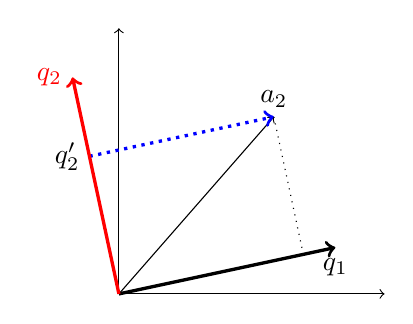
\begin{tikzpicture}[x=8em,y=8em]
    \pgfmathsetmacro{\azx}{1.4}
    \pgfmathsetmacro{\azy}{0.3}
    \pgfmathsetmacro{\aox}{0.7}
    \pgfmathsetmacro{\aoy}{0.8}

    \draw[->] (0,0) -- (1.2,0);
    \draw[->] (0,0) -- (0,1.2);

    \draw[->] (0,0) -- (\aox,\aoy) node[above] {$a_2$};

    \pgfmathsetmacro{\l}{1.0/veclen(\azx,\azy)}
    \pgfmathsetmacro{\qzx}{\azx*\l}
    \pgfmathsetmacro{\qzy}{\azy*\l}

    \draw[very thick,->] (0,0) -- (\qzx,\qzy) node[below] {$q_1$};

    \pgfmathsetmacro{\scal}{\aox*\qzx + \aoy*\qzy}
    \pgfmathsetmacro{\qprjx}{\scal*\qzx}
    \pgfmathsetmacro{\qprjy}{\scal*\qzy}
    \pgfmathsetmacro{\qpox}{\aox - \qprjx}
    \pgfmathsetmacro{\qpoy}{\aoy - \qprjy}
    
    \pgfmathsetmacro{\l}{1.0/veclen(\qpox,\qpoy)}
    \pgfmathsetmacro{\qox}{\qpox*\l}
    \pgfmathsetmacro{\qoy}{\qpoy*\l}

    \draw[dotted, very thick,blue,->] (\qpox,\qpoy) -- (\aox,\aoy);
    \draw[dotted] (\qprjx,\qprjy) -- (\aox,\aoy);

    \draw[very thick,red,->] (0,0) -- (\qox,\qoy) node[left] {$q_2$};
    \draw (\qpox,\qpoy) node[left] {$q'_2$};

  \end{tikzpicture}

  \caption{Gram-Schmidt-Orthogonalisierung. $a_2$ wird in den Vektor
    $q'_2$ transformiert, der zu $q_1$ senkrecht steht, indem die
    Projektion von $q_1$ auf $a_2$ (blau gepunktet) von $a_2$
    abgezogen wird. $q'_2$ wird schließlich noch normiert, um den
    nächsten Basisvektor $q_2$ zu erhalten.}
  \label{fig:gs}
\end{figure}

Das Gram-Schmidt-Verfahren ist das älteste Verfahren zur
QR-Zerlegung. Auf der anderen Seite ist es das allgemeinste Verfahren
und kann in beliebigen Hilberträumen eingesetzt werden. Das Verfahren
ist eigentlich nur eine Orthogonalisierung der Spaltenvektoren von
$A$, die als Nebenprodukt eine QR-Zerlegung liefert. Daher ist das
Verfahren auch als Gram-Schmidt-Orthogonalisierung bekannt. Wir werden
als Beispiel sehen, dass das Verfahren etwa auch zur Konstruktion von
orthogonalen Polynomen eingesetzt werden kann.

Seien zunächst $m$ \emph{linear unabhängige} Vektoren $\{a_j,
j=1(1)m\}$ aus einem beliebigen Hilbertraum $H$ gegeben. Ziel ist es
nun, diese in eine orthonormale Basis $\{q_j, j=1(1)m \}$ zu
transformieren. Wir beginnen mit $a_1$, das wir lediglich normieren
müssen:
\begin{equation}
  q_1 = \frac{a_1}{\norm{a_1}}.
\end{equation}
Den nächsten Vektor, $a_2$, dürfen wir nun nicht einfach normieren und
hinzufügen, da er ja nicht notwendigerweise orthogonal zu $q_1$
ist. Das können wir aber erreichen, indem wir einfach die Anteile
parallel zu $q_1$ abziehen (vergleiche Abbildung~\ref{fig:gs}):
\begin{align*}
  q'_2 &= a_2 - (a_2, q_1)\,q_1\\
  q_2 &= \frac{q'_2}{\norm{q'_2}},
\end{align*}
wobei $(\cdot,\cdot)$ das Skalarprodukt des Hilbertraums $H$
bezeichnet.  Da $a_2$ und $a_1$ nach Voraussetzung linear unabhängig
sein sollen, gilt dies auch für $a_2$ und $q_1$, so dass $q'_2\neq
0$. Mit den weiteren Vektoren verfahren wir genauso, ziehen also
zunächst die Anteile der bereits berechneten Basisvektoren ab und
normieren den Rest:
\begin{align}
  \label{eq:gs}
  q'_k &= a_k - \sum_{i=1}^{k-1} (a_k, q_i)\,q_i\\
  q_k &= \frac{q'_k}{\norm{q'_k}}.
\end{align}
Da wir lineare Unabhängigkeit der $a_i$ vorausgesetzt haben, ist dabei
gesichert, dass $q'_k\neq 0$ für alle $k$. Außerdem gilt
\begin{align}
  (q'_k,q_l) = \left(a_k - \sum_{i=1}^{k-1} (a_k, q_i) q_i, q_l\right) =
  (a_k, q_l) - \sum_{i=1}^{k-1} (a_k, q_i) \underbrace{(q_i,
    q_l)}_{=\delta_{il}} = 0.
\end{align}
Die zu $q'_k$ parallelen $q_k$ sind damit paarweise orthogonal.

Gleichung \eqref{eq:gs} zeigt auch, dass die orthonormale Basis nicht
eindeutig ist, denn wir können genauso gut
$q_k=-\nicefrac{q'_k}{\norm{q'_k}}$ wählen oder, im Falle eines
komplexen Hilbertraums, jeden beliebigen anderen anderen Faktor vom
Betrag 1.

Das Gram-Schmidt-Verfahren benötigt zur Funktion lediglich das
Skalarprodukt des zugrundeliegenden Hilbertraums, und kann daher auch
zur Orthonormalisierung etwa von Polynomen eingesetzt werden, wie wir
gleich sehen werden. Doch zunächst wollen wir uns den Fall ansehen,
dass $A=(a_j)\in\CC^{m,n}$ eine Matrix mit linear unabhängigen Spalten
ist, und die Vektoren $a_j$ deren Spaltenvektoren. Offenbar muss $m\ge
n$ gelten, sonst sind die Spalten linear abhängig. Wir setzen
$Q=(q_j)\in\CC^{m,n}$ die Matrix der mit dem Gram-Schmidt-Verfahren
orthonormierten Spaltenvektoren, und $R=(r_{ik})\in\CC^{n,n}$ mit
\begin{equation}
  r_{ik} =
  \begin{cases}
    (a_k, q_i)  & \text{falls}\; i < k\\
    \norm{q'_k} & \text{falls}\; i = k\\
    0           & \text{sonst}
  \end{cases}
\end{equation}
Dann gilt wegen \eqref{eq:gs}
\begin{equation}
  a_k = q_k\norm{q'_k} + \sum_{i=1}^{k-1} (a_k, q_i) q_i =
  \sum_{i=1}^n  q_i r_{ik}
\end{equation}
und damit $A=QR$ mit $Q^HQ=I$. Ist $m=n$, so ist dann $Q$ die gesuchte
unitäre Matrix und $R$ die rechte obere Dreiecksmatrix der
QR-Zerlegung.

Das Verfahren benötigt bei quadratischen Matrizen genauso wie die
Gauß-Elimination $\O(n^3)$ Schritte, da für jeden Vektor $\O(n)$
Skalarprodukte berechnet werden müssen. Außerdem arbeitet das
Verfahren auf vollen Matrizen, was, wie schon gesagt, bei dünn
besetzten Matrizen ungünstig ist und die Anwendbarkeit bei großen
Matrizen einschränkt. Auch hier gibt es daher alternative Verfahren,
von denen wir gleich die Householder-Spiegelungen und Givensrotationen
kennenlernen werden.

\subsubsection{Beispiel: Legendrepolynome}

Da sich das Gram-Schmidt-Verfahren auf beliebige Hilberträume anwenden
lässt, können wir zum Beispiel den Hilbertraum der Polynome
betrachten, mit dem Skalarprodukt
\begin{equation}
  (f, g) := \int_{-1}^1 f(x)g(x)\, dx.
\end{equation}
Dann sind die Polynome $1,x,x^2,\ldots$ linear unabhängig, da die
Koeffizientendarstellung eines Polynoms ja eindeutig ist. Andererseits
sind diese Polynome aber nicht orthonormal bezüglich $(\cdot,\cdot)$,
da zum Beispiel
\begin{equation}
  (1, x) =  \int_{-1}^1 x\, dx = \frac{1}{2}.
\end{equation}

Wir benutzen nun das Gram-Schmidt-Verfahren, um eine orthogonale Basis
zu erzeugen. Da  $(1, 1) = 2$ ist
\begin{equation}
  q_1 = \frac{1}{\sqrt{2}}
\end{equation}
Weiter ist
\begin{equation}
  q'_2 = x - \left(x, \frac{1}{\sqrt{2}}\right) \cdot \frac{1}{\sqrt{2}} = 
  x
\end{equation}
und damit wegen $(x,x) = \nicefrac{2}{3}$
\begin{equation}
  q_2 = \sqrt{\frac{3}{2}} q'_1 =
  \sqrt{\frac{3}{2}} x.
\end{equation}

Analog erhalten wir
\begin{equation}
  q'_3 = x^2 - \frac{3}{2} (x^2, x) \cdot x - \frac{1}{2}(x^2, 1) \cdot 1 = 
  x^2  - \frac{1}{3}
\end{equation}
und
\begin{equation}
  q_3 = \sqrt{45}{8}\left(x^2  - \frac{1}{3}\right).
\end{equation}
Bis auf Vorfaktoren sind dies die ersten drei Legendrepolynome, die
sich auf diese Weise berechnen lassen. Analog ergeben sich die
Chebyshev-Polynome $T_n$, wenn für dieselbe Basis bezüglich
\begin{equation}
  (f, g)_T := \int_{-1}^1 \frac{f(x)g(x)}{\sqrt{1-x^2}}\, dx
\end{equation}
das Gram-Schmidt-Verfahren durchgeführt wird.

\subsubsection{Modifiziertes Gram-Schmidt-Verfahren}
\index{Gram-Schmidt-Verfahren>modifiziertes}

Numerisch ist das Gram-Schmidt-Verfahren nicht sehr stabil, denn falls
zwei Vektoren $a_j$ beinahe parallel sind, kommt es durch Auslöschung
bei der Berechnung der Projektionen zu großen
Rundungsfehlern. Numerisch besser ist das modifizierte
Gram-Schmidt-Verfahren, bei dem die Projektion eines jeden neu
erzeugten Vektors sofort von allen anderen abgezogen wird. Wir setzen
also $Q^{(0)}=A$ und weiter für $k=1(1)n$:
\begin{align}
  \label{eq:modgs}
  q_k^{(k)} &= q_k^{(k-1)}/r_{kk}\nonumber\\
  q_l^{(k)} &= q_l^{(k-1)} - r_{ki}\,q_k^{(k)}\quad\text{für}\; l>k\\
  q_l^{(k)} &= q_l^{(k-1)} \quad\text{für}\; l<k,\nonumber
\end{align}
mit
\begin{align}
  r_{kk} &= \norm{q_k^{(k-1)}}\nonumber\\
  r_{ki} &= \left(q_l^{(k-1)}, q_k^{(k)}\right) =  \left(a_l, q_k^{(k)}\right).
\end{align}

Der folgende Python-Code führt das modifizierte Gram-Schmidt-Verfahren
auf der Matrix $A$ aus, die schrittweise in die orthonormale Matrix
$Q$ transformiert wird, während $R$ mit berechnet wird. Dadurch, dass
in jedem Schritt der neu berechnete Basisvektor von allen weiteren
abgezogen wird, ist der nächste zu berechnende Vektor $q_k$ bereits
orthogonal zu den bisherigen Basisvektoren und muss lediglich
normalisiert werden:
\lstinputlisting[firstline=10]{gramschmidt.py}

\subsection{\keyword{Householder-Verfahren}}
\index{Householder-Spiegelung}

Wie bereits gesagt, sind unitäre Matrizen nichts anderes als
verallgemeinerte Drehungen und Spiegelungen. Insbesondere ist das
Produkt von unitären Matrizen wieder unitär. Die beiden folgenden
Verfahren zur QR-Zerlegung konstruieren $Q$ daher als Produkt von $l$
einfachen elementaren unitären Matrizen $Q_i$, wobei $l$ vom Verfahren
abhängt, wie auch der Typ der Matrizen $Q_i$. Diese transformieren $A$
schrittweise in rechte obere Dreiecksform:
\begin{equation}
  \label{eq:unitprod}
  Q_l\cdots Q_2Q_1A = R\quad\implies\; A =
  \underbrace{Q_1^H\cdots Q_{l-1}^HQ_l^H}_Q R.
\end{equation}

Bei der QR-Zerlegung mittels Householder-Spiegelungen werden nun $m$
Spiegelungen konstruiert, so dass nacheinander die Spalten von $A$
unterhalb der Diagonalen Null werden, und $A$ auf rechte obere
Dreiecksgestalt transformiert wird. Während also das
Gram-Schmidt-Verfahren die Matrix $A$ in $Q$ transformiert und dabei
$R$ als Nebenprodukt anfällt, wird hier $A$ in $R$ transformiert, und
$Q$ fällt als Nebenprodukt ab. Oft wird $Q$ gar nicht explizit
benötigt, und es ist geschickter, nur die Householder-Spiegelungen zu
speichern, die wir nun zunächst definieren wollen.

\begin{figure}
  \centering
  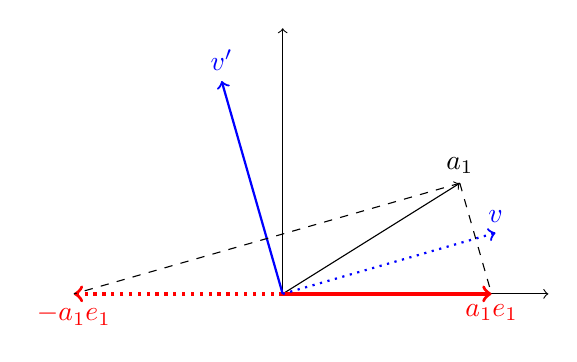
\begin{tikzpicture}[x=8em,y=8em]
    \pgfmathsetmacro{\ax}{0.8}
    \pgfmathsetmacro{\ay}{0.5}

    \pgfmathsetmacro{\l}{veclen(\ax,\ay)}
    \pgfmathsetmacro{\vx}{\ax + \l}
    \pgfmathsetmacro{\vy}{\ay}
    \pgfmathsetmacro{\tmp}{veclen(\vx,\vy)}
    \pgfmathsetmacro{\vx}{\vx/\tmp}
    \pgfmathsetmacro{\vy}{\vy/\tmp}

    \pgfmathsetmacro{\vpx}{\ax - \l}
    \pgfmathsetmacro{\vpy}{\ay}
    \pgfmathsetmacro{\tmp}{veclen(\vpx,\vpy)}
    \pgfmathsetmacro{\vpx}{\vpx/\tmp}
    \pgfmathsetmacro{\vpy}{\vpy/\tmp}

    \draw[->] (0,0) -- (1.2,0);
    \draw[->] (0,0) -- (0,1.2);

    \draw[->] (0,0) -- (\ax,\ay) node[above] {$a_1$};

    \draw[very thick, red, ->] (0,0) -- (\l,0) node[below] {$\norm{a_1} e_1$};

    \draw[very thick, red, dotted, ->] (0,0) -- (-\l,0) node[below] {$-\norm{a_1} e_1$};

    \draw[thick, blue, dotted, ->] (0,0) -- (\vx,\vy) node[above] {$v$};

    \draw[thick, blue, ->] (0,0) -- (\vpx,\vpy) node[above] {$v'$};

    \draw[dashed] (\ax,\ay) -- (-\l, 0);
    \draw[dashed] (\ax,\ay) -- ( \l, 0);

  \end{tikzpicture}

  \caption{Illustration der Householder-Konstruktion. Der Vektor $a_1$
    soll mittels einer Spiegelung auf einen der Vektoren
    $\pm\norm{a_1}e_1$ abgebildet werden. Die zugehörigen
    Householdervektoren sind dann gerade die beiden Winkelhalbierenden
    $v=a+\norm{a_1}e_1$ und $v'=a-\norm{a_1}e_1$. Bei der Spiegelung
    von $v$ wird $a_1$ auf $\norm{a_1} e_1$ abgebildet (durchgezogene
    Linien), bei Spiegelung von $v'$ auf $-\norm{a_1} e_1$
    (gestrichelte Linien).}
  \label{fig:householder}
\end{figure}

Sei also $v\in\RR^m$ ein Vektor mit $\norm{v}^2_2=v^Hv=1$. Dann ist die
zugehörige Householder-Spiegelung definiert als
\begin{equation}
  S_v = I - 2vv^H
\end{equation}
Ist $w = \lambda v$, so gilt $S_vw = w - 2vv^Hw = -w$, $w$ wird also
an der Null gespiegelt. Ist hingegen $w\perp v$, also $v^Hw=0$, dann
ist $S_vw = w$. $S_v$ lässt also die zu $v$ senkrechte Hyperebene
invariant, während Vektoren parallel zu $v$ gespiegelt werden.
Außerdem gilt $S_v^H = S_v$ und $S_v^HS_v = I - 4vv^H + 4vv^Hvv^H =
I$, damit auch $S_v^2=I$, und $S_v$ ist unitär.

Wie können wir nun eine Householder-Spiegelung konstruieren, so dass
diese die erste Spalte $a_1$ von $A$ auf die erste Koordinatenachse
abbildet? Wie man sich leicht überlegt, muss dann $v$ eine der beiden
Winkelhalbierenden sein (vergleiche
Abbildung~\ref{fig:householder}). Diese sind von der Form
\begin{equation}
  v = \frac{a_1 + \lambda e_1}{\norm{a_1 +\lambda e_1}}
\end{equation}
mit
\begin{equation}
  \lambda = \pm\norm{a_1}.
\end{equation}
Für die numerische Stabilität ist es günstiger, Auslöschungen zu
vermeiden, daher wählt man
\begin{equation}
  \lambda = \text{sgn}(a_{11}) \norm{a_1},
\end{equation}
wobei $\text{sgn}(a_{11})$ das Vorzeichen von $a_{11}$ bezeichnet.
Durch die Wahl dieses Vorzeichens ist der unnormierte Spiegelvektor
\begin{equation}
  \tilde{v}_j = \begin{cases}
    \text{sgn}(a_{11})(\abs{a_{11}} + \norm{a_1}_2) & \text{für}\; j=1\\
    a_j & \text{für}\; j>1,
  \end{cases}
\end{equation}
so dass es zu keiner Auslöschung kommen kann. Der eigentliche
Spiegelvektor ist der normierte Vektor $v =
\tilde{v}/\norm{\tilde{v}}_2$.

Bei der Implementation ist es natürlich wichtig, $S_v$ \emph{nicht}
explizit zu berechnen. Es gilt aber
\begin{equation}
  \label{eq:hhupdate}
  S_vA = A - 2v v^HA = A - 2 v (v^HA)
\end{equation}
Man berechnet also lediglich einmal den Vektor $t = v^HA$, und zieht
dann das $t_j$-fache von $v_j$ von der Spalte $a_j$ ab. Um weitere
Spalten von $A$ auf rechte obere Dreiecksform zu bringen, fixieren wir
die bereits bearbeiteten Koordinaten, und betrachten nur noch eine
Spiegelung in den verbleibenden Koordinaten. Dann sieht für die $k$-te
Spalte der unnormierte Spiegelvektor so aus:
\begin{equation}
  \tilde{v}^{(k)}_j = \begin{cases}
    0 & \text{für} j < k\\
    \text{sgn}(a_{kk})(\abs{a_{kk}} + \sqrt{\sum_{l = k}^m a_l^2}) & \text{für}\; j=k\\
    a_j & \text{für}\; j>k,
  \end{cases}
\end{equation}
und der normierte Spiegelvektor ist $v^{(k)} =
\tilde{v}^{(k)}/\norm{\tilde{v}^{(k)}}_2$. Die Wurzel entspricht der
Norm des Restvektors $(a_{kk},\ldots,a_{mk})$. Nach $\min(m,n)-1$
Schritten ist dann $A$ auf Dreiecksform transformiert.

Um die Matrix $Q$ zu erhalten, müssen wir gemäß \eqref{eq:unitprod}
das Produkt der Spiegelungen in umgekehrte Reihenfolge berechnen, da
ja $S_v = S_v^H$. Wurden nacheinander die Spiegelungen mit Vektor
$v_1, v_2,\ldots,v_{l}$ angewandt, suchen wir also die Matrix
\begin{equation}
  Q = S_{v^{(1)}}^HS_{v^{(2)}}^H\cdots S_{v^{(l)}}^H =
  = I\,S_{v^{(1)}}S_{v^{(2)}}\cdots S_{v^{(l)}}.
\end{equation}
Um diese zu berechnen, müssen wir nur die Identität von rechts mit den
Spiegelungen multiplizieren, was analog \eqref{eq:hhupdate} geht:
\begin{equation}
  \label{eq:hhupdateh}
  AS_v  = A - 2Av v^H = A - 2(Av) v^H.
\end{equation}
Vielfach ist es aber gar nicht nötig, $Q$ explizit zu kennen, dann
kann man einfach die Vektoren $v^{(k)}$ speichern und bei Bedarf $Qw$
für einen beliebigen Vektor $w$ ausrechnen, indem die Spiegelungen in
umgekehrter Reihenfolge auf $w$ angewandt werden.

In Python könnte eine QR-Zerlegung mittels Householder-Spiegelungen
so aussehen:
\lstinputlisting[firstline=10]{householder.py}
Die Funktionen \lstinline!multiplyleft! und \lstinline!multiplyright!
implementieren \eqref{eq:hhupdate} bzw. \eqref{eq:hhupdateh}, die
Hauptschleife muss also nur den Spiegelvektor $v^{(k)}$ berechnen und
auf $R$ und $Q$ entsprechend anwenden.

Ist $A$ nicht quadratisch oder singulär, dann müssen unter Umständen
Spalten getauscht werden, wenn die gesamte führende Spalte der
aktuellen Restmatrix Null ist. Spaltentauschmatrizen sind ebenfalls
unitäre, selbstinverse Matrizen, werden allerdings von rechts
anmultipliziert. Anders als das Gram-Schmidt-Verfahren kann das
Householder-Verfahren also auf beliebige Matrizen angewandt
werden. Man erhält dann eine allgemeine Zerlegung
\begin{equation}
  A = Q \cdot \begin{pmatrix}
    R' & K \\
    0 & 0
  \end{pmatrix} \cdot S,
\end{equation}
wobei $R'$ eine reguläre rechte obere Dreiecksmatrix ist, $Q$ das
unitäre Produkt der Householder-Spiegelungen und $S$ die unitäre
Matrix der eventuell nötigen Spaltenvertauschungen.

Jedes Matrix-Update gemäß \eqref{eq:hhupdate} benötigt im wesentlichen
$\O(nm)$ Operationen, die Methode insgesamt daher $\O(mn^2)$
Operationen, bei quadratischen Matrizen also wie auch das
Gram-Schmidt-Verfahren $\O(n^3)$ Schritte.

Die QR-Zerlegung mit Hilfe von Householder-Spiegelungen ist in SciPy
als \scipy{scipy.linalg.qr(A)} implementiert und liefert die Zerlegung
$Q$ und $R$ zurück. Wird das Schlüsselwortargument \argd{pivoting} auf
\texttt{True} gesetzt, werden zusätzlich noch Spalten getauscht und
die neuen Spaltenindizes zusätzlich zurückgegeben.

\subsection{Givens-Rotationen}
\index{Givens-Rotation}

Spiegelungen sind prinzipiell Operationen, die die gesamte Matrix
betreffen, wie \eqref{eq:hhupdate} zeigt. Wie das
Gram-Schmidt-Verfahren ist daher auch das Householder-Verfahren nicht
für dünn besetzte Matrizen geeignet und schlecht zu
parallelisieren. Daher setzt man in der Praxis gerne Givens-Rotationen
ein.

Eine Givensrotation ist eine Drehung in zwei Koordinaten, also eine
Matrix der Gestalt:
\begin{equation}
  G_{i,k,\phi} = \begin{matrix}
    \\
    i\rightarrow\\
    \\
    k\rightarrow\\
    \\
  \end{matrix}\begin{pmatrix}
    I      & 0 & \ldots& 0&0\\
    0      & c & 0 & s & 0 \\
    \vdots & 0 & I & 0 & \vdots\\
    0      & -s & 0 & c & 0 \\
    0      & 0 & \ldots& 0 &I
  \end{pmatrix}
\end{equation}
mit $c=\cos(\phi)$ und $s=\sin(\phi)$ und einem beliebigen Winkel
$\phi$. Die beiden Cosinusterme befinden sich stets auf der
Diagonalen. Offenbar ist $G_{i,k,\phi}$ eine unitäre Matrix, als
$G_{i,k,\phi}^HG_{i,k,\phi}=I$.

\begin{figure}
  \centering
  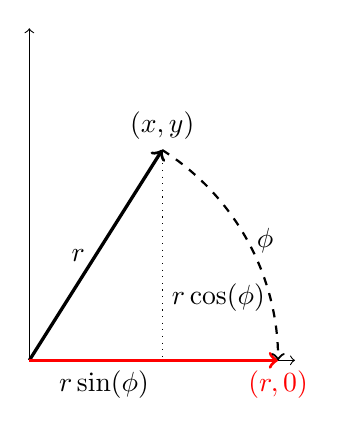
\begin{tikzpicture}[x=8em,y=8em]
    \pgfmathsetmacro{\ax}{0.6}
    \pgfmathsetmacro{\ay}{0.95}

    \pgfmathsetmacro{\l}{veclen(\ax,\ay)}
    \pgfmathsetmacro{\a}{atan(\ay/\ax)}

    \pgfmathsetmacro{\cx}{\l*cos(\a/2)}
    \pgfmathsetmacro{\cy}{\l*sin(\a/2)}

    \draw[->] (0,0) -- (1.2,0);
    \draw[->] (0,0) -- (0,1.5);

    \draw[dotted] (\ax,\ay) -- node[right,pos=0.7] {$r\cos(\phi)$} (\ax,0);

    \draw[very thick, ->] (0,0) -- node[left] {$r$} (\ax,\ay) node[above] {$(x,y)$};

    \draw[very thick, red, ->] (0,0) -- node[below,pos=0.3,black] {$r\sin(\phi)$} (\l,0) node[below]
    {$(r, 0)$};
    
    \draw[thick, dashed, ->] (\ax,\ay) arc (\a:0:\l);
    \draw (\cx,\cy) node[right] {$\phi$};
  \end{tikzpicture}

  \caption{Illustration der Givens-Konstruktion. Der Vektor $(x,y)$
    soll um den Winkel $\phi$ auf die $x$-Achse gedreht werden. Dann
    gilt $\cos(\phi) = \nicefrac{x}{r}$  und $\sin(\phi) =
    \nicefrac{x}{r}$ mit $r=\sqrt{x^2+y^2}$.}
  \label{fig:givens}
\end{figure}

Wir können nun eine solche Drehung benutzen, um das linke untere
Element $a_{n,1}$ einer Matrix $A$ auf $0$ zu bekommen. Dazu drehen
wir die beiden untersten Zeilen der Matrix entsprechend:
\begin{equation}
  \begin{pmatrix}
    I & 0 & 0\\
    0 & c  & s\\
    0 & -s  & c
  \end{pmatrix}
  \cdot
  \begin{pmatrix}
    \vdots & \ddots\\
    x & \ldots\\
    y & \ldots
  \end{pmatrix}
  \stackrel{!}{=}
  \begin{pmatrix}
    \vdots & \ddots\\
    r & \star\\
    0 & \star
  \end{pmatrix}
\end{equation}
mit $x=a_{n-1,1}$ und $y=a_{n,1}$ sowie $r=\sqrt{x^2 + y^2}$.  Die
Sterne deuten dabei an, dass sich die gesamten beiden letzten Zeilen
potentiell ändern. Den Drehwinkel muss man dabei gar nicht explizit
bestimmen, da $c=\cos(\phi) = x/r$ und $s=\cos(\phi) = y/r$
(vergleiche Abbildung~\ref{fig:givens}).

Ist $r$ allerdings klein, ist diese Formel numerisch nicht stabil. Im
Falle, dass $\abs{x}\ge\abs{y}$, berechnet man daher besser
\begin{align}
  \label{eq:calccs}
  r'&=\sqrt{1 + \left(\nicefrac{y}{x}\right)^2}\nonumber\\
  c &=\text{sgn}(x)\frac{1}{r'}\\
  s &= \frac{y}{\abs{x}r'}\nonumber,
\end{align}
und analog im
umgekehrten Falle.

Nachdem wir nun das linke unterste Element $a_{n,1}$ auf Null gedreht
haben, können wir mit dem nächsthöheren Element $a_{n-1,1}$ fortfahren
und dieses auf $a_{n-2,1}$ drehen. Wir fahren fort, bis die erste
Spalte mit Ausnahme des ersten Elements auf Nullen gedreht ist. Analog
können wir nun in den folgenden Spalten unten anfangend alle Elemente
bis auf das Diagonalelement auf Null drehen.

Auch die Givens-Rotationen werden dabei nicht als
Matrix-Multiplikation berechnet, da sich bei Multiplikation von links
tatsächlich ja nur zwei Zeilen lesen und neu schreiben. Für die
Berechnung von $Q$ müssen wir nach \eqref{eq:unitprod} die hermiteschen der
Rotationen von rechts anmultiplizieren, was einer Modifikation zweier
Spalten entspricht. Die Hermitesche bzw. Transponierte der Drehung
ergibt sich einfach durch Drehung in der umgekehrten Richtung, also
Vorzeichenwechsel des Sinusterms.

\clearpage

In Python sieht das Givens-Verfahren so aus:
\lstinputlisting[firstline=10]{givens.py}
Die Routinen \lstinline!multiplyleft! und \lstinline!multiplyright!
implementieren wieder die Multiplikation mit einer Givensmatrix von
links bzw.\ rechts. Die Routine \lstinline!calccs! implementiert die
stabilisierte Berechnung der Sinus- und Cosinusterme gemäß \eqref{eq:calccs}.

Bei einer vollbesetzten Matrix benötigt das Verfahren damit insgesamt
$\O(mn)$ Drehungen, die allerdings jeweils nur zwei Zeilen der Matrix
verändern, also $\O(n)$ Rechenaufwand haben. Daher benötigt das
Verfahren insgesamt wieder $\O(mn^2)$.

Anders als das Householder-Verfahren eignen sich Givensrotationen aber
auch für parallele Verarbeitung und dünn besetzte Gitter. Denn für das
Verfahren ist es im Prinzip egal, auf welche Zeile die zu entfernende
gedreht wird, es müssen ja nicht notwendigerweise benachbarte Zeilen
sein. Daher reicht es, nur die besetzten Elemente unterhalb der
Diagonalen jeweils nacheinander auf die Diagonale drehen. Bei der
$5\times 5$-Matrix des Eingangsbeispiels \eqref{eq:laplacedisc} sind
daher lediglich 50 statt 300 Drehungen nötig.

\section{Eigenwerte}
\index{Eigenwert}
\index{Eigenvektor}

In der Quantenmechanik spielt die Berechnung von Eigenwerten- und
vektoren, also von Eigenenergien und -zuständen, eine zentrale Rolle.

Gegeben ist wieder eine Matrix $A\in\RR^{n,n}$. Wir suchen
nichttriviale Vektoren $v\in\RR^n$ und Skalare $\lambda$, so dass
\begin{equation}
  Av = \lambda v \quad\iff\quad (A-\lambda I)v = 0.
\end{equation}
Die Formulierung auf der rechten Seite zeigt, dass für alle Eigenwerte
$\lambda$ die Matrix $A-\lambda I$ singulär sein muss, also
\begin{equation}
  \det (A-\lambda I) = 0.
\end{equation}
Die Determinante ist aber letztlich nichts weiter als ein Polynom
$n$-ten Grades in $\lambda$, dessen Nullstellen gerade die Eigenwerte
sind. Das Newtonverfahren konvergiert für Polynome, so dass wir mit
seiner Hilfe die Eigenwerte im Prinzip bestimmen können.

Das Problem ist, dass $\lambda$ eine Variable ist, so dass wir nicht
auf die QR- oder LU-Zerlegung zurückgreifen können. Wir müssen also
die Matrix zum Beispiel entlang der ersten Zeile entwickeln, und $n$
Unterdeterminanten der Größe $n-1$ berechnen. Diese wiederum erfordern
$n-1$ Unterdeterminanten der Größe $n-2$, und so weiter. Ingesamt also
sind $n!$ viele Unterteilungsschritte nötig, was selbst bei moderat
großen Matrizen nicht handhabbar ist und außerdem schnell zur
Anhäufung von Fehlern führt. Daher wird dieses einfache Variante nur
bei Matrizen in bis zu vier Dimensionen genutzt, für größere Matrizen
hingegen Näherungsverfahren, die wir nun kennen lernen werden.

\subsection{\keyword{Vektoriteration}}

Sei die Matrix $A$ zunächst diagonalisierbar, also
$A=Q\,\text{diag}(\lambda_1,\ldots,\lambda_n)Q^H$ mit einer unitären Matrix
$Q$. Dann gilt für eine beliebigen Vektor $x^{(0)}\neq 0$
\begin{equation}
  \tilde{x}^{(i)} := A^i x^{(0)} = Q\,\text{diag}(\lambda_1,\ldots,\lambda_n)^i Q^H x^{(0)}
  = \sum_{k=1}^n (q_k, x^{(0)}) \lambda_k^i q_k.
\end{equation}
Ist nun $\abs{\lambda_1}>\abs{\lambda_k}$ für alle $k>1$, also der
betragsmäßig größte Eigenwert $\lambda_1$ nicht entartet, so ist
$\lambda_1^i\gg\lambda_k^i$ für große $i$. Daher wird $\tilde{x}_i$
mit wachsender Anzahl Iterationen zunehmend parallel zu einem
Eigenvektor zu $\lambda_1$. Allerdings wird dabei $\tilde{x}_i$
gleichzeitig immer größer bzw.\ kleiner, wenn $\abs{\lambda_1}$ größer
bzw.\ kleiner 1 ist. Um numerische Probleme zu vermeiden, muss
$\tilde{x}_i$ noch normiert werden.

Dies führt zum Verfahren der Vektoriteration oder von-Mises-Iteration.
Man wählt einen Startvektor $x^{(0)}\neq 0$, und berechnet dann
iterativ
\begin{equation}
  x^{(i+1)} = \frac{A x^{(i)}}{\norm{A x^{(i)}}_2}.
\end{equation}
Hat die Matrix $A$ einen nicht entarteten betragsmäßig größten
Eigenwert, so konvergiert $x^{(i)}$ gegen einen dazugehörigen
Einheitseigenvektor, falls $x^{(0)}$ nicht gerade exakt senkrecht auf
dem Eigenraum steht. In der Praxis ist dies aufgrund numerischer
Ungenauigkeiten wenigstens für eine der Iterierten immer der
Fall. Außerdem konvergiert $\left(x^{(i)}\right)^HAx^{(i)}$ gegen
diesen Eigenwert.

Ist der betragsmäßig größte Eigenwert entartet, aber es gibt keine
weiteren Eigenwerte mit gleichem Betrag, so konvergiert
$\left(x^{(i)}\right)^HAx^{(i)}$ immer noch gegen den betragsmäßig größten
Eigenwert. Gibt es mehrere betragsgleiche, aber unterschiedliche
größte Eigenwerte (etwa $\pm 1$), konvergiert dieses Verfahren nicht.

Das Verfahren konvergiert vergleichsweise langsam, und findet nur den
betragsmäßig größten Eigenwert. Man könnte zwar versuchen, den neuen
Startwert durch Orthogonalisierung senkrecht zum Eigenraum des größten
Eigenvektors zu wählen, aber im Allgemeinen verhindern wieder numerische
Ungenauigkeiten, dass das Verfahren gegen einen anderen Eigenwert
konvergiert.

Zumindest einen weiteren Eigenwert kann man finden, indem man die
\emph{geshiftete} Matrix $A - \lambda_1I$ betrachtet, für die
$\lambda_1$ notwendigerweise dem betragsmäßig kleinsten Eigenwert,
nämlich 0, entspricht. Der gefundene Eigenwert $\mu_1$ entspricht
einen Eigenwert $\lambda_1 + \mu_1$ der Ursprungsmatrix $A$.

\subsubsection{Beispiel: Fibonaccizahlen}

Die Fibonaccizahlen sind definiert als $F_0 = 0$, $F_1=1$ und
$F_{i+2} = F_{i+1} + F_i$ für $i \ge 0$. Dies lässt sich auch als
Vektoriteration schreiben:
\begin{equation}
  \begin{pmatrix}
    F_0\\
    F_1
  \end{pmatrix}=
  \begin{pmatrix}
    0\\
    1
  \end{pmatrix}
  \quad\text{und}\;
  \begin{pmatrix}
    F_{i+1}\\
    F_{i+2}
  \end{pmatrix}=
  \underbrace{\begin{pmatrix}
      0 & 1\\
      1 & 1
    \end{pmatrix}}_A\cdot
  \begin{pmatrix}
    F_i\\
    F_{i+1}
  \end{pmatrix}.
\end{equation}
In diesem Fall ist es natürlich möglich, die Eigenwerte und -vektoren
von $A$ analytisch zu bestimmen. Die Eigenwerte sind die Nullstellen
\begin{equation}
  \det(A-\lambda I) = -\lambda(1-\lambda) - 1 = \left(\lambda
    -\frac{1}{2}\right)^2 - \frac{5}{4},
\end{equation}
also $\lambda_{\pm} = \frac{1}{2} \left(1 \pm \sqrt{5}\right)$. Davon
ist $\lambda_+ > 1$ der größere Eigenwert, und $\lambda_-<1$. Die
dazugehörigen Eigenvektoren sind
\begin{equation}
  x_{\pm} =
  \begin{pmatrix}
    1\\
    \frac{1}{2} \left(1 \pm
      \sqrt{5}\right)
  \end{pmatrix}.
\end{equation}
Der Startwert $(0,1)^T$ der Fibonaccireihe ergibt sich in der Basis
der Eigenvektoren als
\begin{equation}
  x_0 = 
  \begin{pmatrix}
    0\\
    1
  \end{pmatrix} =
  \frac{1}{\sqrt{5}} x_+ - \frac{1}{\sqrt{5}} x_-.
\end{equation}
Betrachten nun die $x$-Komponente von $A^ix_0$, können wir die
Fibonaccizahlen auch als
\begin{equation}
  F_i = \frac{1}{\sqrt{5}}\lambda_+^i + \frac{1}{\sqrt{5}}\lambda_-^i
  = \frac{1}{\sqrt{5}} \left(\frac{1 + \sqrt{5}}{2}\right)^i
  - \frac{1}{\sqrt{5}} \left(\frac{1 - \sqrt{5}}{2}\right)^i \in\NN
\end{equation}
schreiben. Insbesondere ist $F_i = \O_{i\to\infty}\left(\left(\frac{1
      + \sqrt{5}}{2}\right)^i\right)$, unabhängig davon, welche
Startwerte benutzt werden, solange diese nicht gerade parallel zu
$x_-$ sind. Für ganzzahlige Startwerte ist dies nur möglich, wenn
$F_0=F_1=0$. 

\subsection{\keyword{QR-Algorithmus}}

Da die Vektoriteration nicht alle Eigenwerte und -vektoren liefert,
brauchen wir noch ein anderes Verfahren, das alle Eigenwerte berechnen
kann. Dieser Abschnitt führt hierzu den QR-Algorithmus von Francis und
Kublanovskaya ein.

Grundlage dieses iterativen Algorithmus ist, wie der Name schon sagt,
die QR-Zerlegung. Wir starten mit $A^{(0)} = A\in\CC^{n,n}$. In jedem
Iterationsschritt berechnen wir eine QR-Zerlegung
$A^{(k)}=Q^{(k)}R^{(k)}$, und setzen
\begin{equation}
  A^{(k+1)} = R^{(k)}Q^{(k)} = \left(Q^{(k)}\right)^HA^{(k)}Q^{(k)}.
\end{equation}
Die letztere Umformung zeigt, dass $A^{(k+1)}$ dieselben Eigenwerte wie
$A^{(k)}$ und damit auch $A$ hat. Konvergiert dieses Verfahren,
bedeutet dies, dass $Q^{(k)}\approx I$ für große $k$, und damit ist
$A^{(k+1)}$ nahezu rechte obere Dreiecksmatrix, deren Eigenwerte wir
von der Diagonalen ablesen können. Hat $A$ keine entarteten
Eigenwerte, so konvergieren die $A^{(k)}$ sogar gegen eine
Diagonalmatrix. Dies gilt allerdings nur, solange der Algorithmus über
komplexen Matrizen durchgeführt wird, die stets eine Schursche
Normalform haben. Der reellwertige Algorithmus hingegen führt nur zu
einer Matrix mit $2\times 2$-Blöcken auf der Diagonalen, die jeweils
zwei komplex konjugierten Eigenwerten über $\CC$ entsprechen.

Eine einfache Erweiterung des Verfahrens zerlegt nicht $A^{(k)}$,
sondern $A^{(k)} - \mu_kI = \tilde{Q}^{(k)}\tilde{R}^{(k)}$, wobei $\mu_k$ eine
Näherung für einen Eigenwert ist. Oft wird einfach $\mu_k = a_{n,n}$
gewählt. Die nächste Iterierte ist dann
\begin{equation}
  A^{(k+1)} = \tilde{R}^{(k)}\tilde{Q}^{(k)} + \mu_kI,
\end{equation}
der Shift wird also einfach wieder rückgängig gemacht.

Der Algorithmus benötigt sehr viele, teure QR-Zerlegungen. Um den
Rechenaufwand zu vermindern, kann man die Matrix zunächst durch
Householder-Spiegelungen auf Hessenberg-Form bringen, die dann mit
Hilfe von Givens-Rotationen sehr schnell QR-zerlegt werden kann.

Eine einfache Implementation des QR-Algorithmus mit Shift für eine
Matrix mit reellen Eigenwerten kann wie folgt aussehen:
\lstinputlisting[firstline=10]{qr.py}
Die Routine liefert einen Vektor aus Eigenwerten mit Hilfe des
Householder-Verfahrens von SciPy. \argd{tolerance} gibt dabei den
maximalen Betrag eines Subdiagonalelements an, der noch akzeptiert
wird.  Hat \argd{A} komplexe Eigenwerte, können auch Element eins
unter der Diagonalen nicht verschwinden. Dann muss zum einen
das Kriterium muss dann entsprechend angepasst werden, zum zweiten
kann dann natürlich nicht einfach die Diagonale zurückgeliefert
werden. Echte, also reelle Eigenwerte sind dann solche, die weder
links noch unterhalb auf der Subdiagonalen Nachbarn haben, die anderen
entsprechen komplexen Eigenwerten.

\subsection{Inverse Iteration}
\index{inverse Iteration}

Die Eigenvektoren ergeben sich im Prinzip aus dem Produkt aller
$Q^{(k)}$. Einfacher ist es aber, eine sogenannte inverse Iteration
durchzuführen. Ist $\lambda$ eine gute Approximation eines Eigenwerts
$\lambda_0$ der Matrix $A\in\CC^{n,n}$, so ist $\mu = (\lambda_0
-\lambda)^{-1}$ ein sehr großer Eigenwert von $(A-\lambda I)^{-1}$,
und der Eigenvektor $v$ zu $\mu$ ist auch ein Eigenvektor von $A$ zu
$\lambda$. Ist zum Beispiel $\lambda$ eine auf 5 Stellen genaue
Näherung, so ist $\abs{\mu}\approx 100.000$.

Da $\mu$ sehr groß ist, konvergiert die Vektoriteration für
$(A-\lambda I)^{-1}$ sehr schnell. Dazu wird natürlich nicht die
Inverse berechnet, sondern man startet wie gewohnt mit einem Startwert
$x^{(0)}\neq 0$ und löst
\begin{equation}
  (A - \lambda I) \tilde{x}^{(i+1)} = x^{(i)}
\end{equation}
durch Gaußelimination mit Pivotisierung. Die neue Iterierte wird noch
normiert:
\begin{equation}
  x^{(i+1)} = \frac{\tilde{x}^{(i+1)}}{\norm{\tilde{x}^{(i+1)}}_2}.
\end{equation}
Bei einer sehr guten Eigenwertnäherung oder auch durch kleine
numerische Fehler kann es passieren, dass das Pivotelement der
Gaußelimination numerisch exakt Null ist. In diesem Fall wird es
einfach durch eine sehr kleine Zahl ersetzt. Da letztlich nur die
Richtung ausschlaggebend ist, konvergiert dieses Verfahren extrem
schnell gegen den zu $\lambda$ gehörigen Eigenvektor.

Die inverse Iteration, die zu einem gegebenen nicht-entarteten
Eigenwert den Eigenvektor bestimmt, sieht wie folgt aus:
\lstinputlisting[firstline=10]{inverse_iteration.py}
\argd{l} ist hier der Eigenwert $\lambda$, zu dem der Eigenvektor
gesucht wird. Hier gibt die Toleranz an, wie sehr $Ax$ von $\lambda x$
abweichen darf.

\subsubsection{Beispiel: Fibonaccizahlen numerisch}

Der QR-Algorithmus mit Shift $a^{(k)}_{n,n}$ soll nun anhand des
Fibonaccibeispiels illustriert werden, für das dieser Algorithmus sehr
schnell konvergiert, wie die folgende Tabelle illustriert:
\begin{center}
  \renewcommand{\arraystretch}{1.3}
  \begin{tabular}{r|c|c|c}
    Iteration & $A^{(k)}$ & Stellen $\lambda_+$ &  Stellen $\lambda_-$\\
    0 & $\begin{pmatrix}
      0.00000000 &  1.00000000\\
      1.00000000 &  1.00000000
    \end{pmatrix}$
    & 0 & 0\\
    1 & $\begin{pmatrix}
      -0.50000000 &  0.50000000\\
      0.50000000 & 1.50000000
    \end{pmatrix}$
    & 0 & 0\\
    2 & $\begin{pmatrix}
      -0.61764706 &  0.02941176\\
      0.02941176 & 1.61764706
    \end{pmatrix}$
    & 3 & 3\\
    3 & $\begin{pmatrix}
      -0.61803399 &  0.00000509\\
      0.00000509 & 1.61803399
    \end{pmatrix}$
    & 10 & 10\\
    4 & $\begin{pmatrix}
      -0.61803399 & -0.00000000\\
      0.00000000 & 1.61803399
    \end{pmatrix}$ & 15 & 17
  \end{tabular}
\end{center}
Die letzten beiden Spalten geben die Anzahl der korrekt bestimmten
Nachkommastellen des größten bzw.\ kleinsten Eigenwerts an. Nach dem
vierten Schritt verbessert sich daran nichts mehr, da beide Eigenwerte
bis auf Maschinengenauigkeit bestimmt sind.  Um die zugehörigen
Eigenvektoren zu bestimmen, können wir die inverse Iteration benutzen,
die in diesem Fall für beide Eigenvektoren innerhalb von nur einem
Schritt auf Maschinengenauigkeit konvergiert.

Wie sieht es nun mit größeren Matrizen aus? Ist eine Matrix
$A\in\RR^{10,10}$ symmetrisch mit Standardzufallszahlen gefüllt,
konvergiert das Verfahren in etwa 200 Schritten so, dass unterhalb der
Diagonalen keine Werte betragsmäßig größer als $10^{-5}$ stehen. Auch
hier konvergiert die inverse Iteration innerhalb eines Schritts
praktisch bis auf Maschinengenauigkeit gegen den zugehörigen
Eigenvektor.

%%% Local Variables: 
%%% mode: latex
%%% TeX-master: "padc.tex"
%%% TeX-PDF-mode: t
%%% End: 
